\subsection{MetaDE}
MetaDE package implements 12 major meta-analysis methods for differential expression analysis, and now it allows the analysis of both microarray and RNA-seq data. In this tutorial, we will demonstrate the MetaDE pipeline step by step using two meta-analysis methods: Fisher's method and Adaptively weighted Fisher's method (AW-Fisher). Please refer to \cite{fisher1925statistical} and \cite{li2011adaptively} for details of these two methods. 
Individual MetaDE package is also available on GitHub at \url{https://github.com/metaOmic/MetaDE}.


\subsubsection{Meta analysis}

After opening the MetaDE page, as shown in Figure \ref{fig:MetaDEmainpage}, there are 2 drop-down menus (``Meta Method Type" and ``Meta Method") and 4 tabs on the left of the page (``Response Type", ``Setting Individual Study Method", ``Advanced Options" and ``Run"). We generally suggest users not to change any parameter setting in the ``Advanced Options" unless users know the underlying methodology well. 

\begin{figure}[H]
\begin{center}
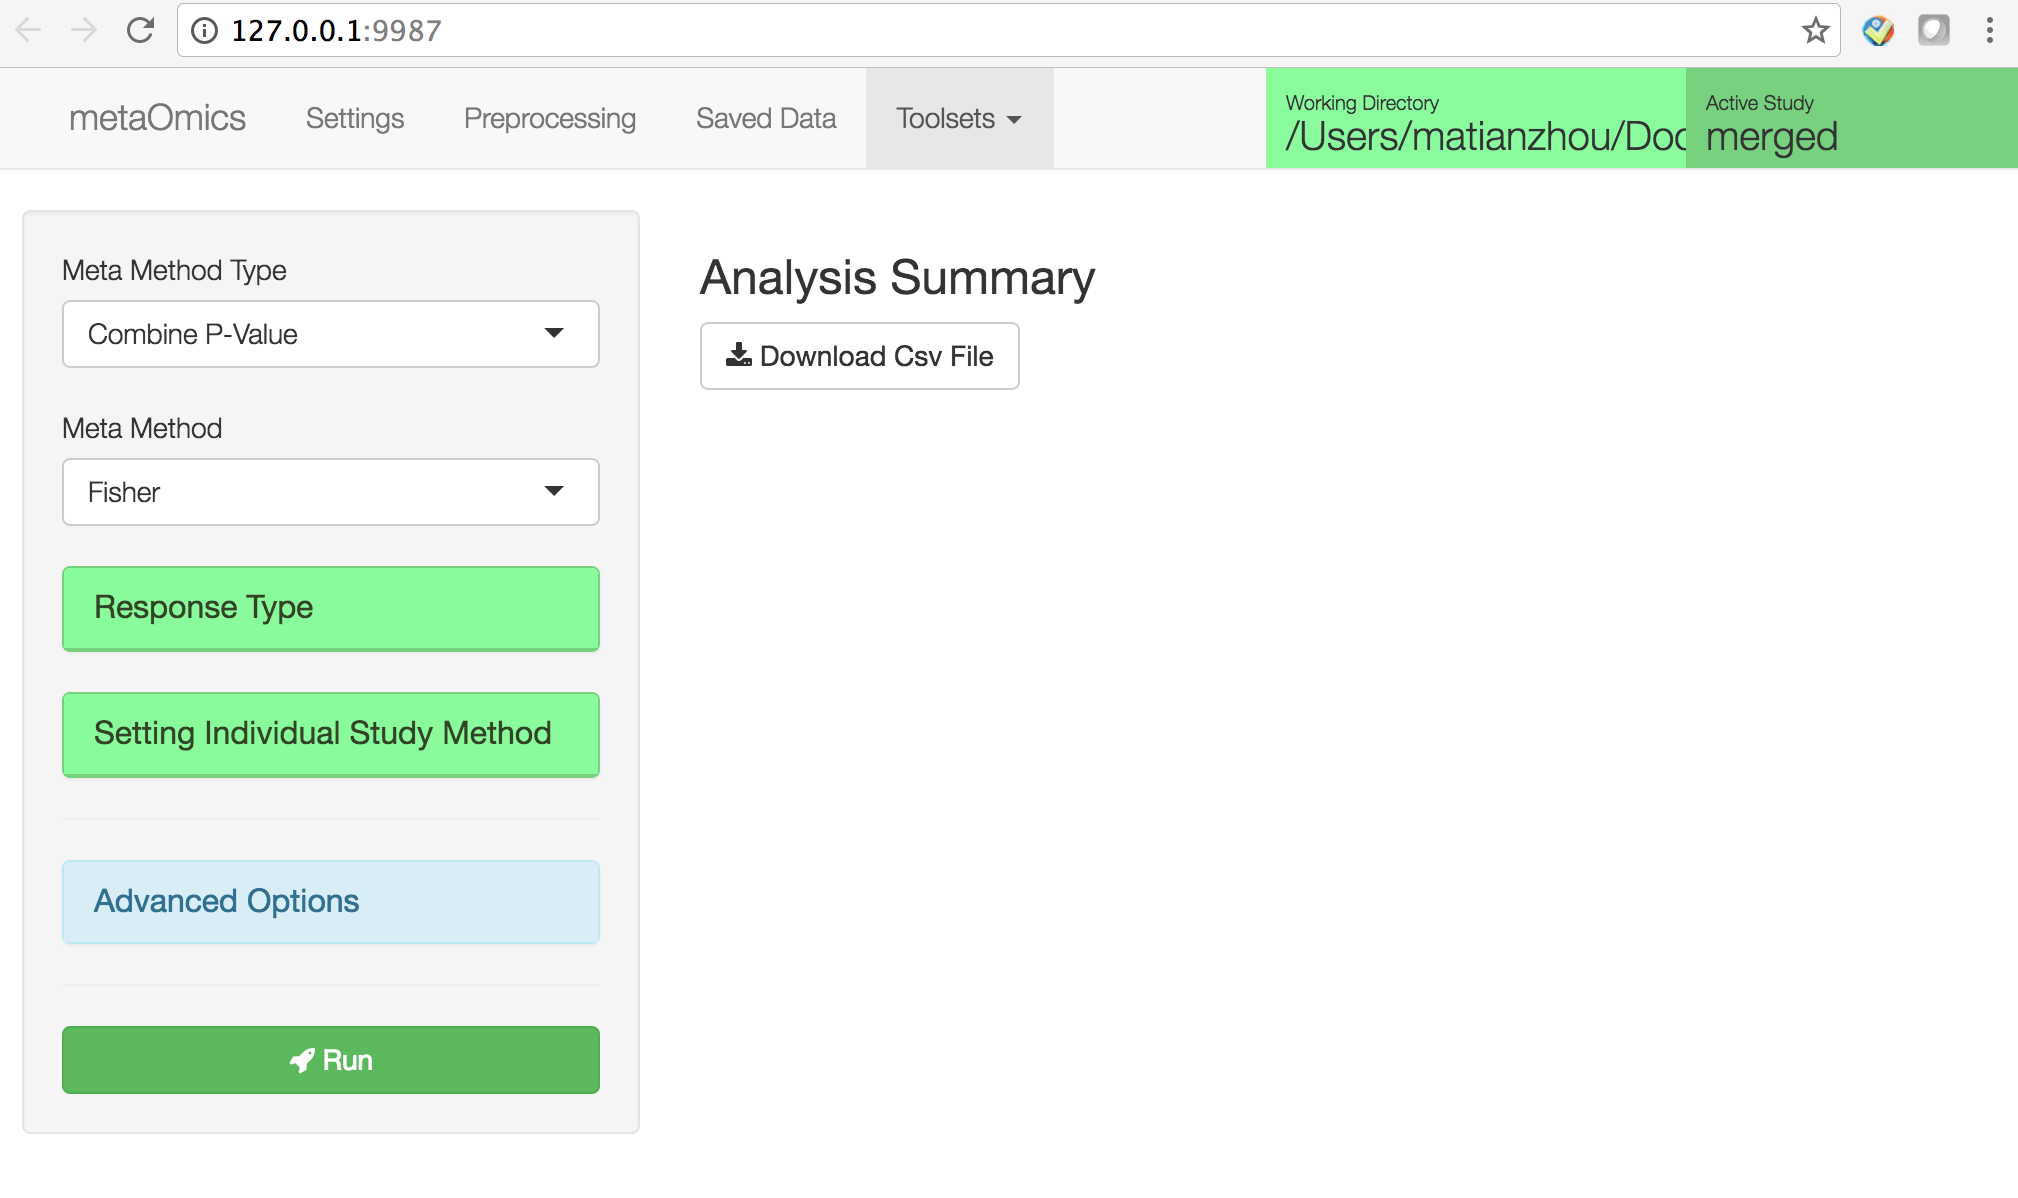
\includegraphics[scale=0.45]{./figure/metaDE/MetaDEmainpage}
\caption{Homepage of MetaDE}
\label{fig:MetaDEmainpage}
\end{center}
\end{figure}

For Fisher's method, we will choose ``Combine P-value" and ``Fisher" (Figure \ref{fig:FisherSelect}); and for AW Fisher's method, we will choose ``Combine P-value" and ``AW Fisher" (Figure \ref{fig:AWFisherSelect}). 

\begin{figure}[H]
\begin{center}
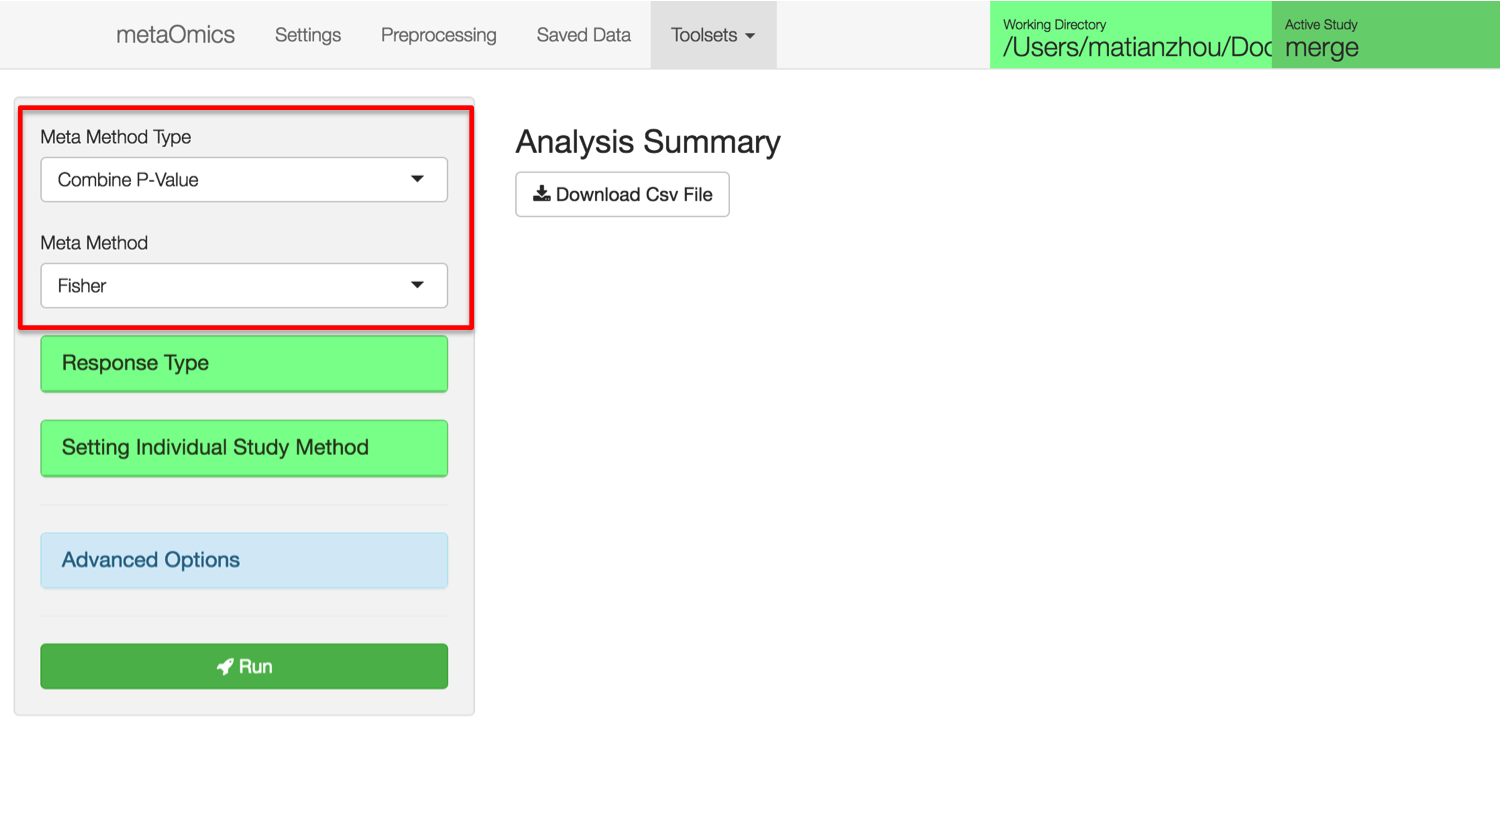
\includegraphics[scale=0.45]{./figure/metaDE/FisherSelect}
\caption{Fisher's method setting}
\label{fig:FisherSelect}
\end{center}
\end{figure}

\begin{figure}[H]
\begin{center}
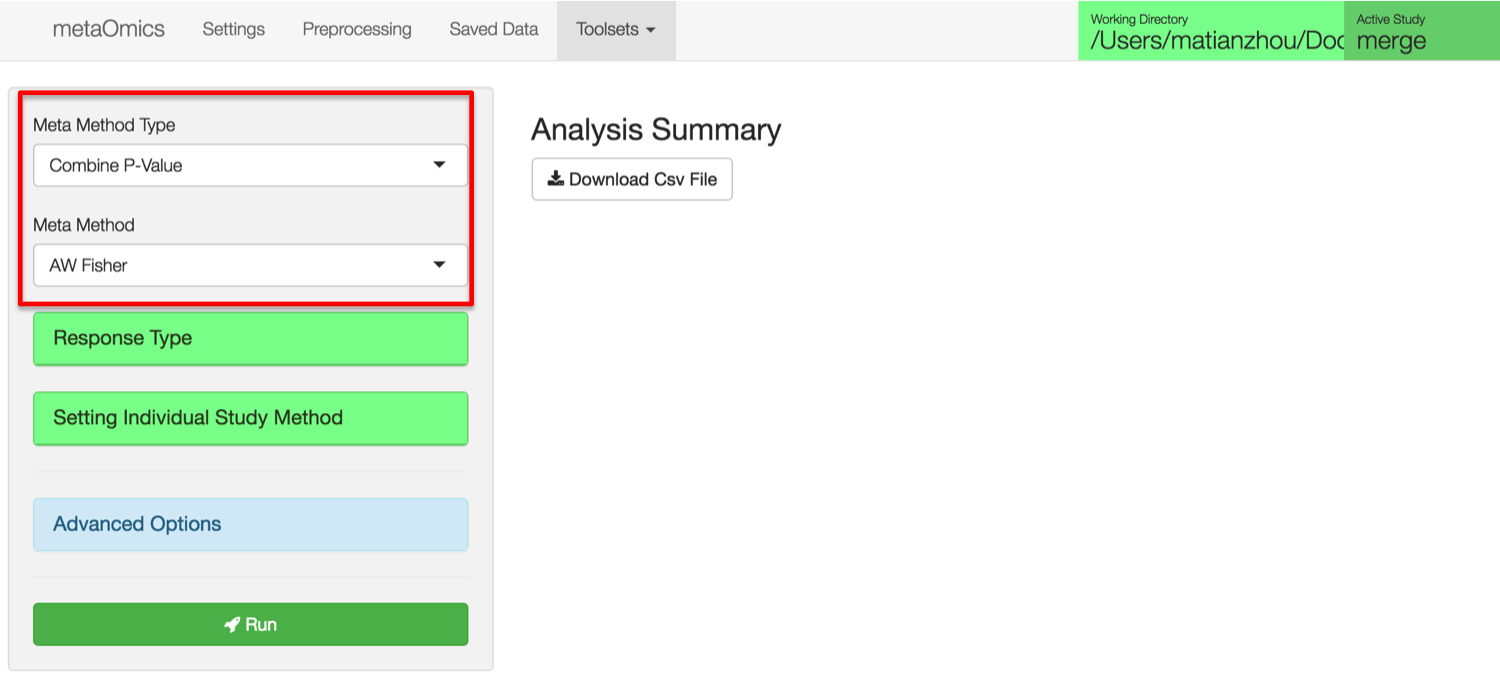
\includegraphics[scale=0.45]{./figure/metaDE/AWFisherSelect}
\caption{AW Fisher's method setting}
\label{fig:AWFisherSelect}
\end{center}
\end{figure}

Then, in the next step, we click on ``Response Type", for two-class DE analysis, choose ``Two Class Comparison", choose the group label name for the Label Attribute (from the column names of your clinical data). Then for the group label (a factor of at least two levels), choose a name for the ``Control Label" and ``Experimental Label", respectively (Figure \ref{fig:ResponseType}).

\begin{figure}[H]
\begin{center}
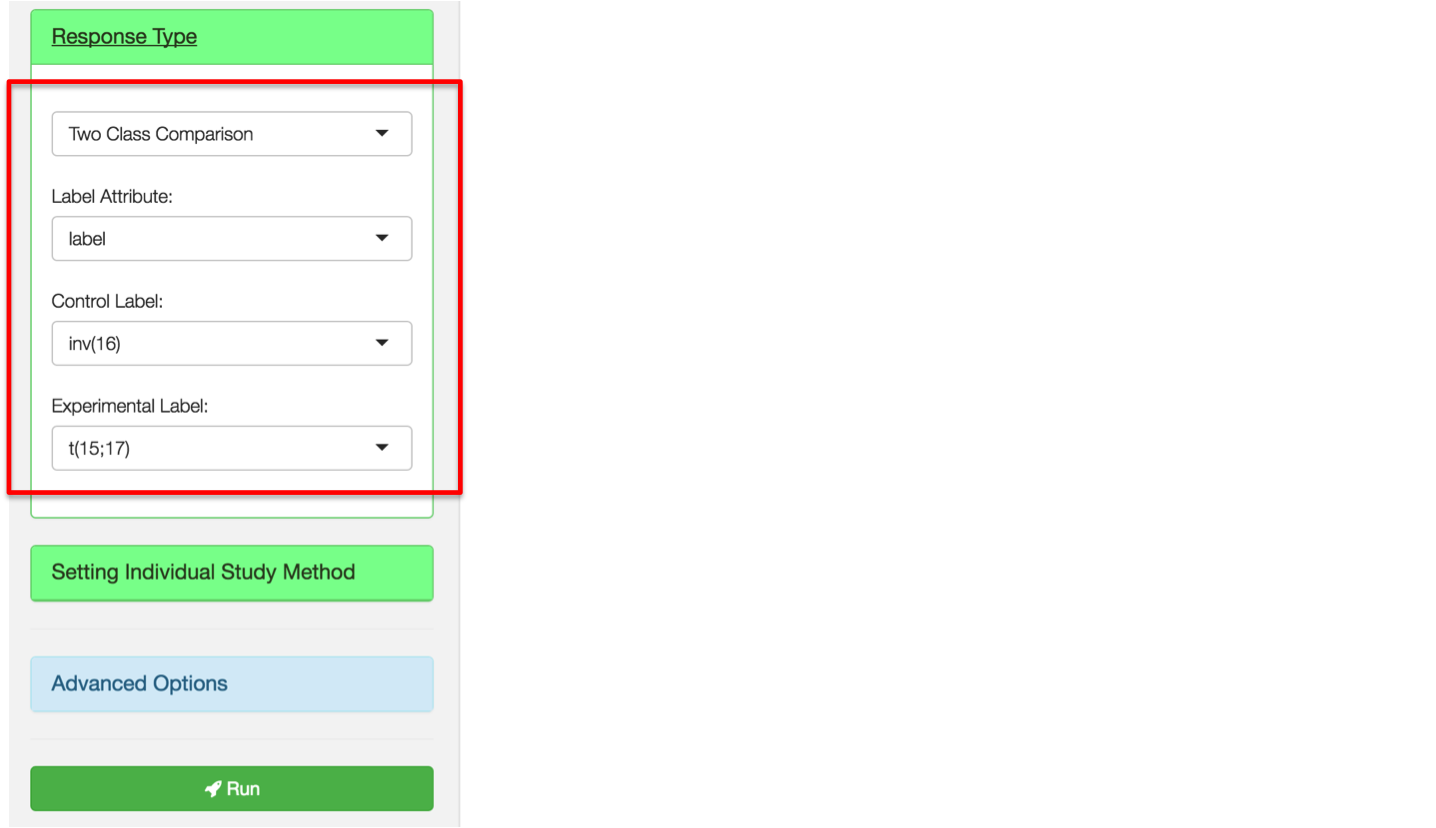
\includegraphics[scale=0.45]{./figure/metaDE/ResponseType}
\caption{Response type setting}
\label{fig:ResponseType}
\end{center}
\end{figure}

Next, we click on ``Setting Individual Study Method" and choose ``LIMMA" to perform DE analysis in each individual study (Figure \ref{fig:IndDE}). Available options include ``LIMMA" and ``SAM" for continuous data (e.g. microarray), ``edgeR", ``DESeq2" and ``limmaVoom" for discrete data (e.g. RNA-seq count). Details of the above mentioned DE methods can be found in XXX (reference).

\begin{figure}[H]
\begin{center}
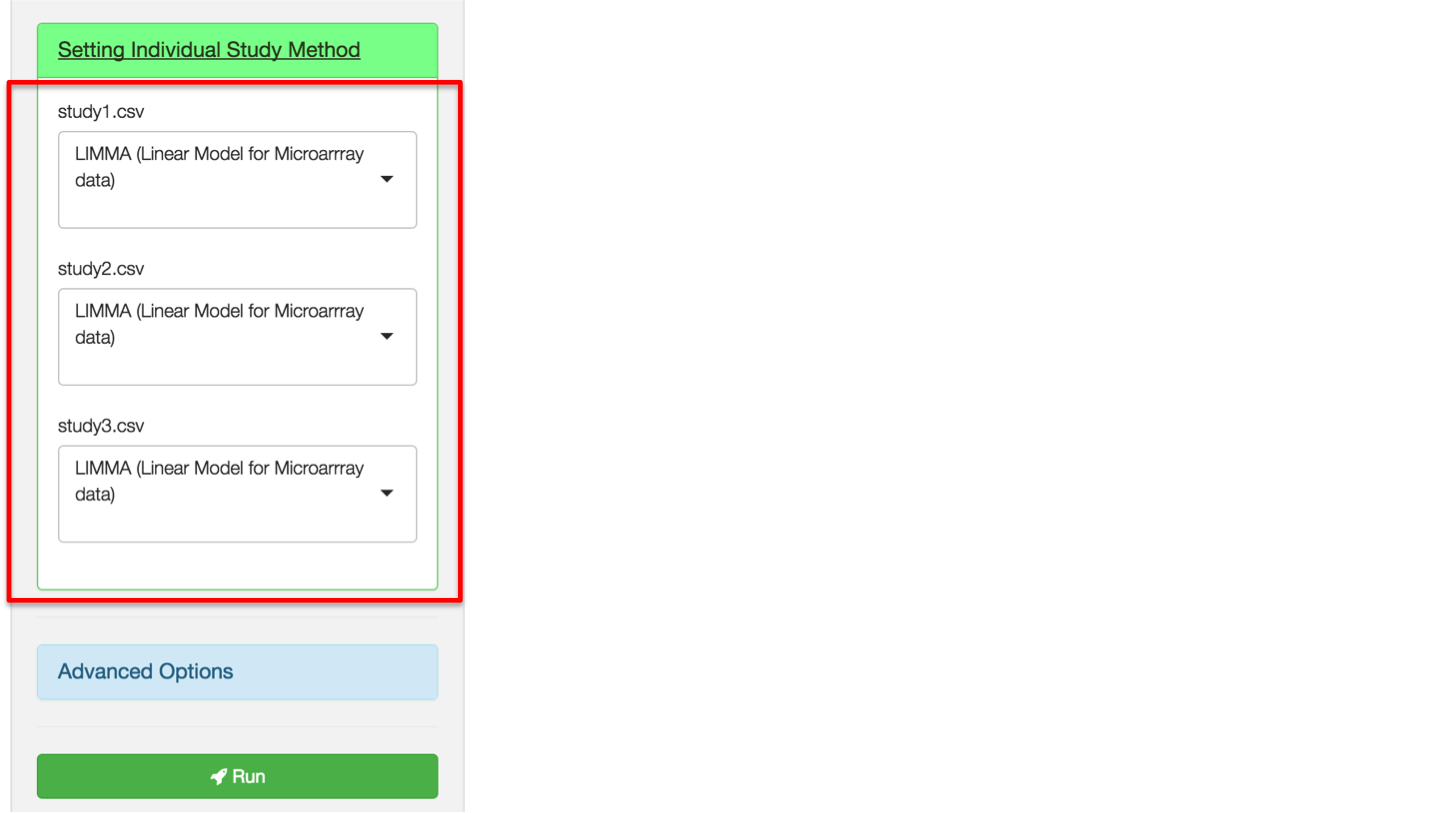
\includegraphics[scale=0.45]{./figure/metaDE/IndDE}
\caption{Individual study DE analysis method}
\label{fig:IndDE}
\end{center}
\end{figure}

** Optionally, we can click on ``Advanced Options", choose ``Parametric=yes" so parametric methods will be used for inference. We can choose whether to adjust for any important ``Covariates" (e.g. potential confounders) and we set the alternative hypothesis to be ``abs", i.e. two-sided test (Figure \ref{fig:AdvOptions}). 

\begin{figure}[H]
\begin{center}
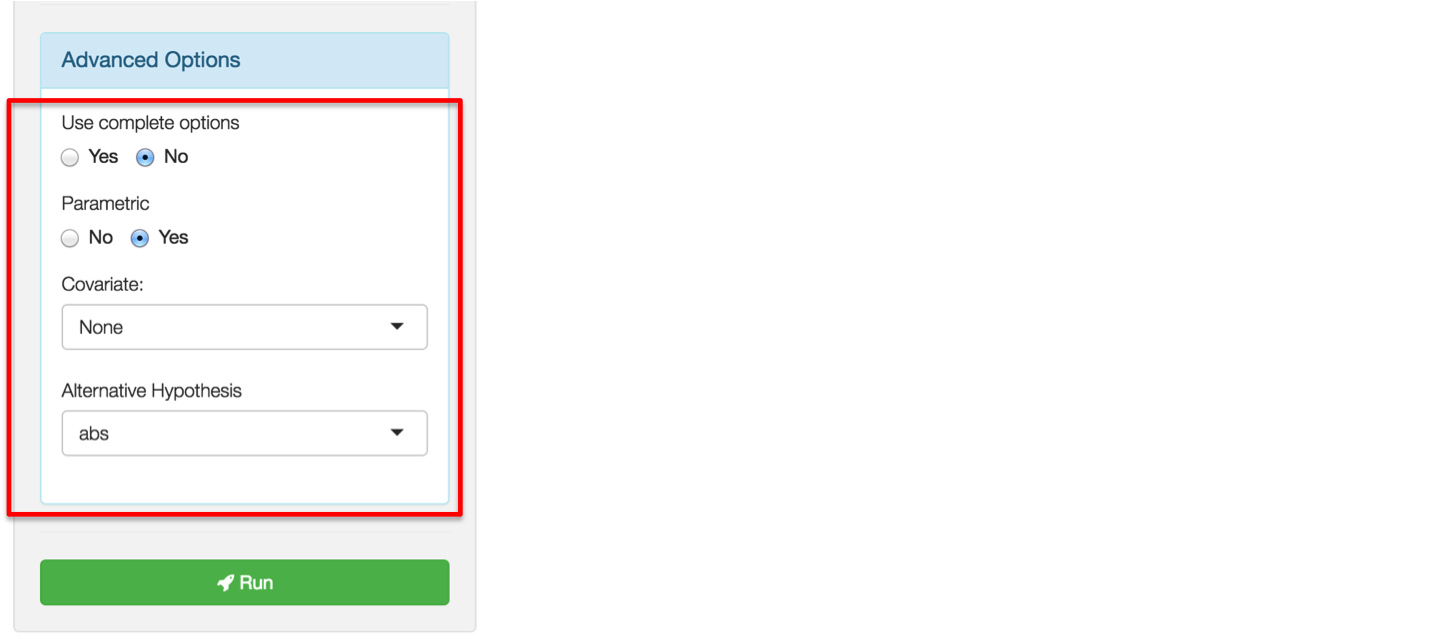
\includegraphics[scale=0.45]{./figure/metaDE/AdvOptions}
\caption{Advanced Options}
\label{fig:AdvOptions}
\end{center}
\end{figure}

After we click on ``Run", we will see a summary table generated on the right of the page as shown in Figure \ref{fig:MetaSummary}. The ``Analysis Summary" includes the analysis results of all genes, including individual study statistics/p-value, meta-analysis statistics/p-value/FDR, etc. Users can search the gene name in the ``Search" bar, and download the full table as a csv file by clicking on ``Download Csv File".  

\begin{figure}[H]
\begin{center}
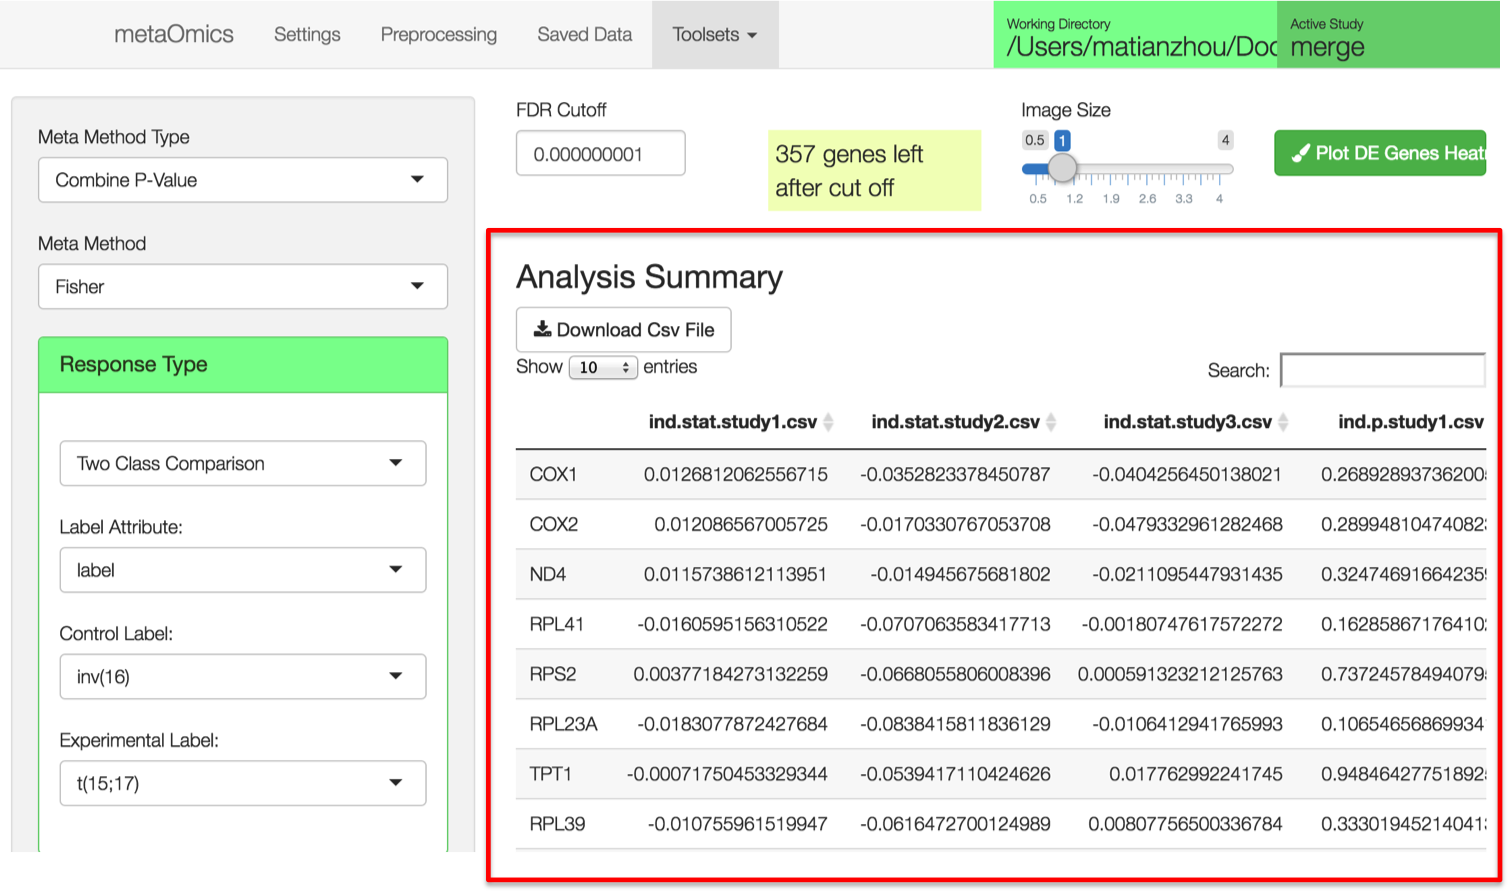
\includegraphics[scale=0.45]{./figure/metaDE/MetaSummary}
\caption{Summary table of Meta-analysis results}
\label{fig:MetaSummary}
\end{center}
\end{figure}

\subsubsection{Visualization}

In addition to tabular output, for better visualization, users can also plot heatmap of DE genes at specified FDR cutoff. Users can enter the ``FDR Cutoff" (number of genes selected are shown interactively), then click on ``Plot DE Genes Hetamap" to draw the heatmap. The ``image size" can be adjusted by dragging the scroll bar (Figure \ref{fig:HeatmapSetting}).  

\begin{figure}[H]
\begin{center}
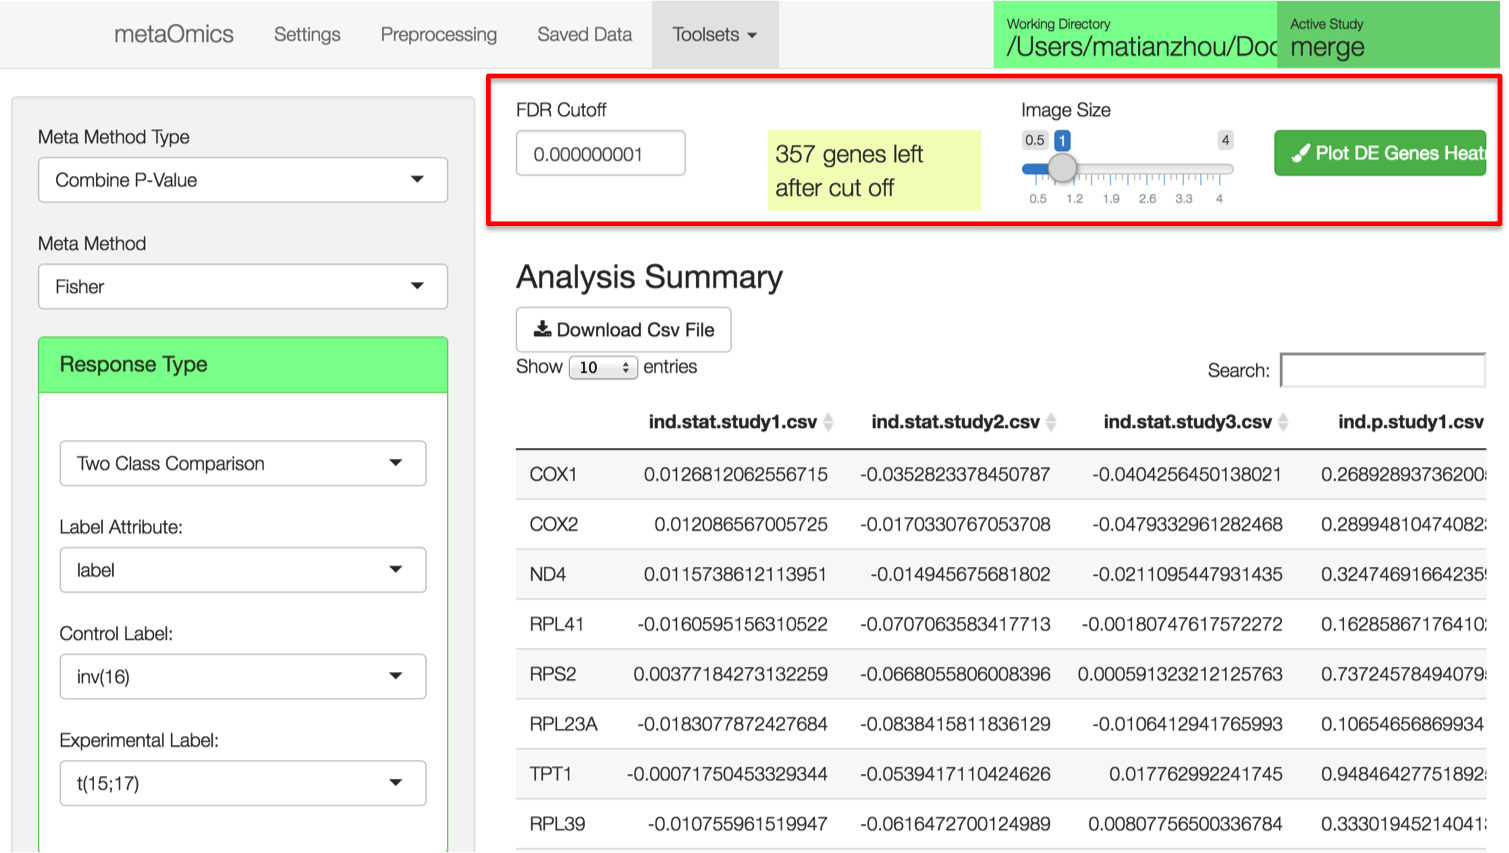
\includegraphics[scale=0.4]{./figure/metaDE/HeatmapSetting.png}
\caption{Plot heatmap setting}
\label{fig:HeatmapSetting}
\end{center}
\end{figure}

Shown in Figure \ref{fig:FisherHeatmap} and Figure \ref{fig:AWFisherHeatmap} are two heatmaps generated from Fisher and AW Fisher results. Note that one additional column of weight distribution across studies is added in the heatmap of AW-Fisher, and all genes in the heatmap are sorted based on their weight distribution.

\begin{figure}[H]
\begin{center}
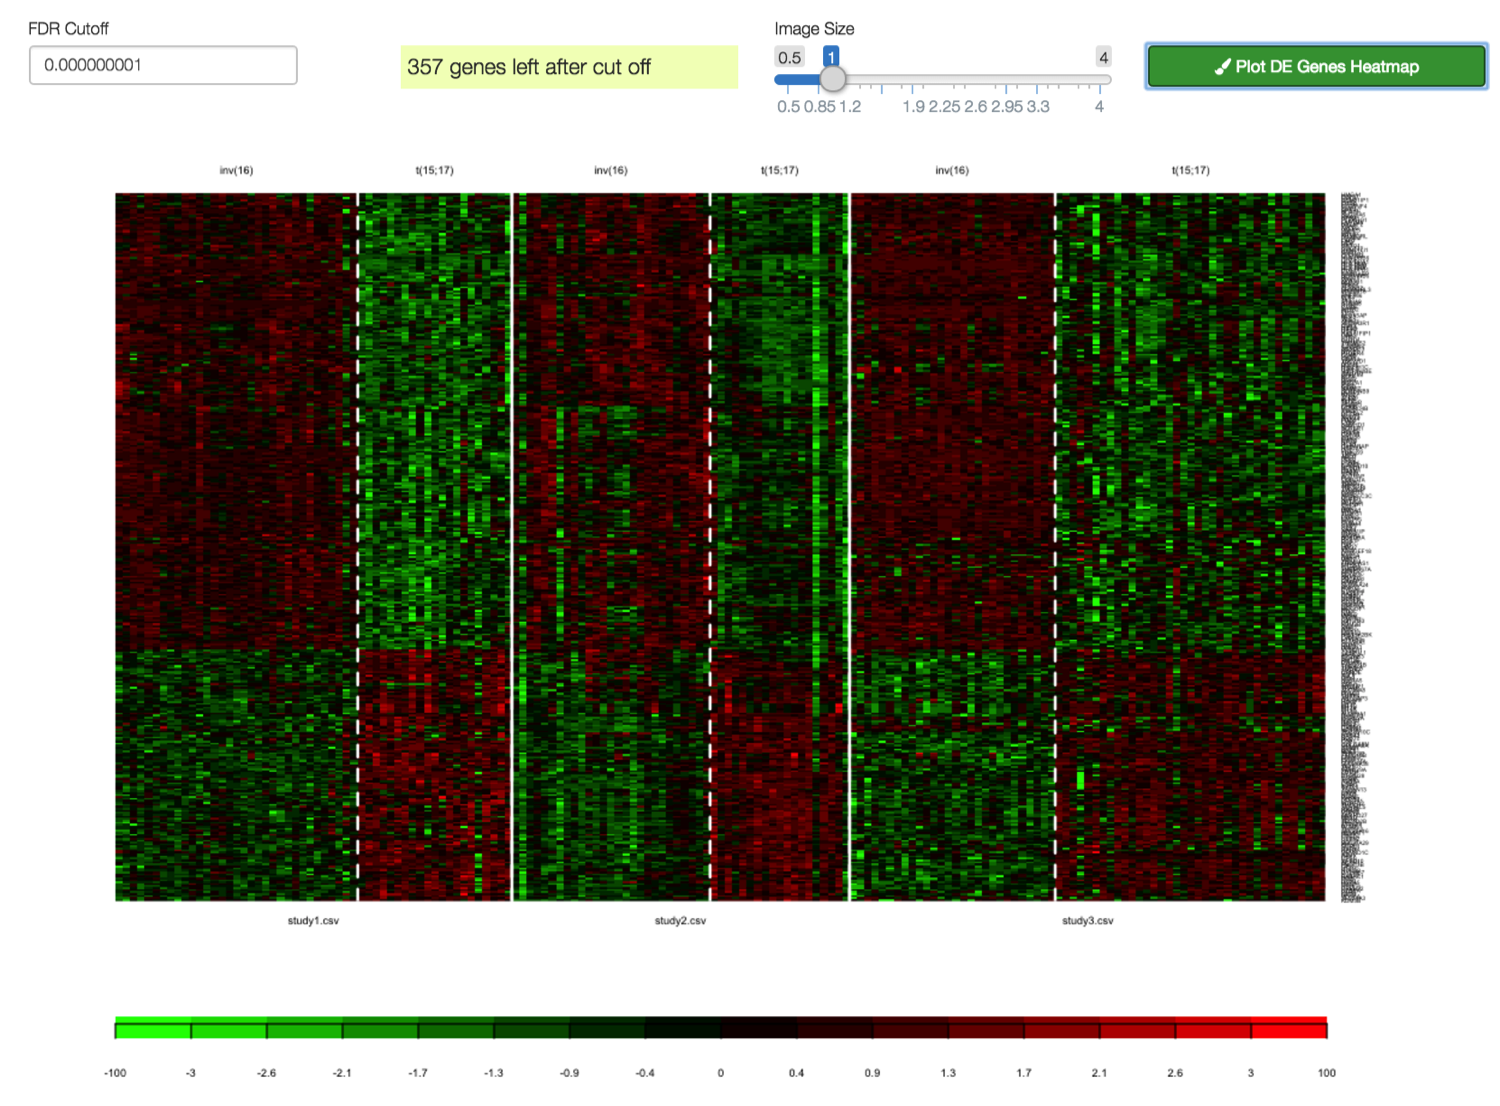
\includegraphics[scale=0.4]{./figure/metaDE/FisherHeatmap}
\caption{Heatmap based on Fisher results}
\label{fig:FisherHeatmap}
\end{center}
\end{figure}

\begin{figure}[H]
\begin{center}
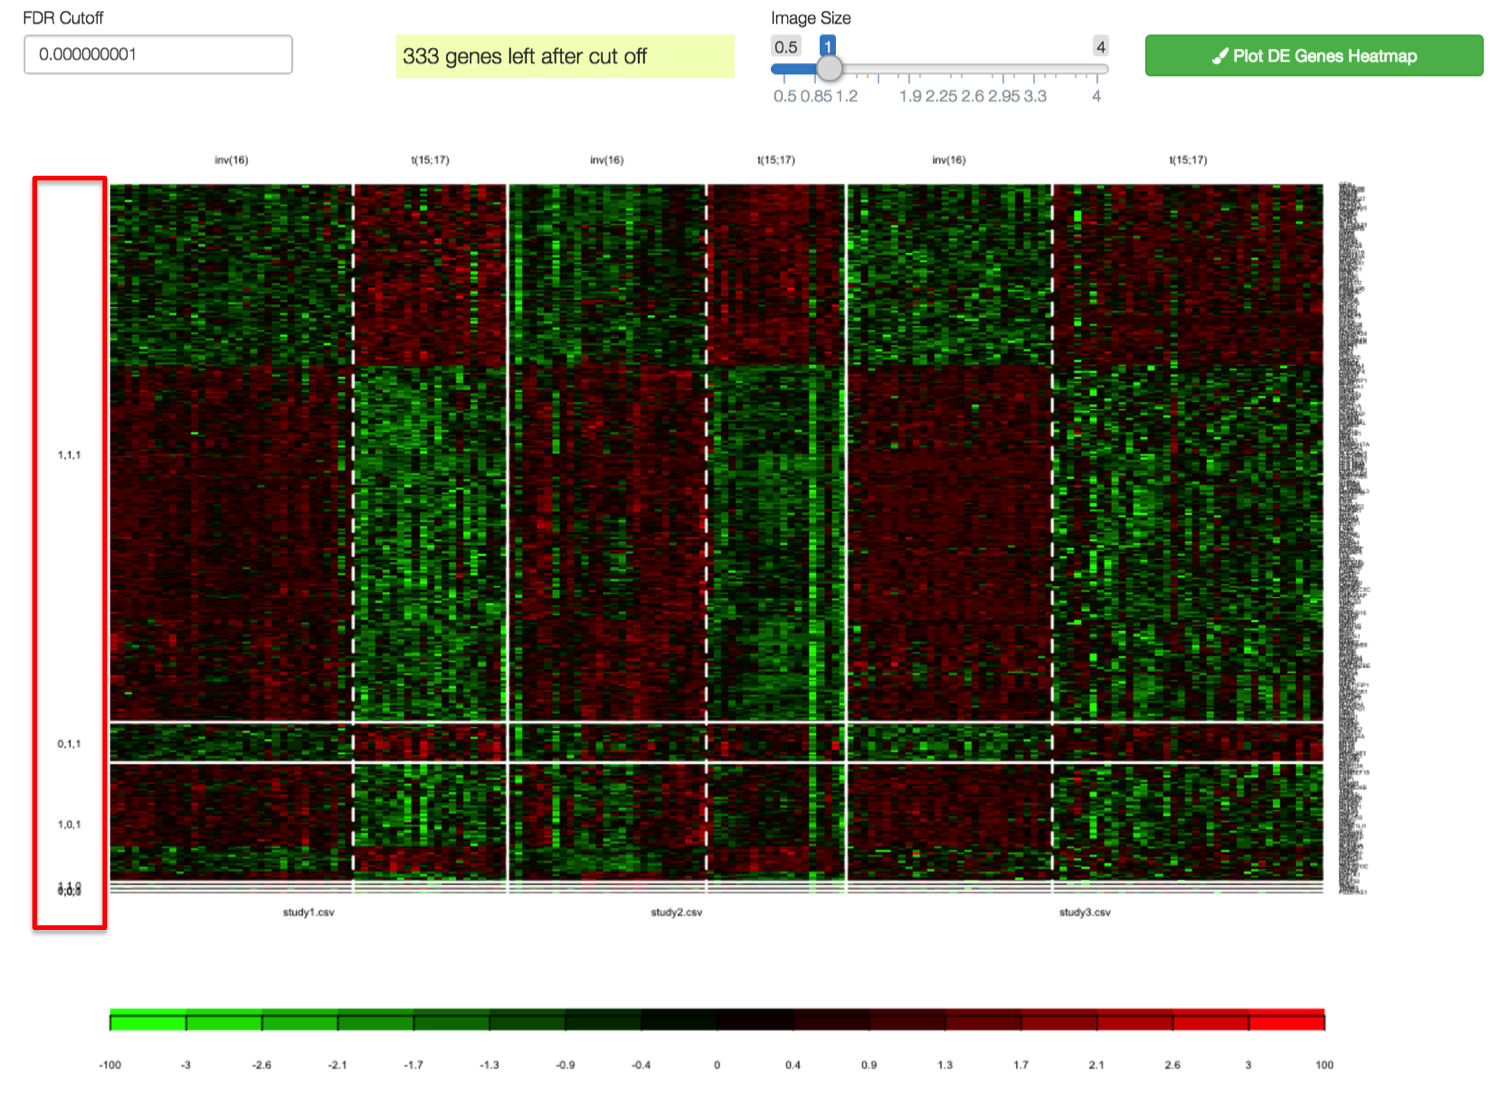
\includegraphics[scale=0.45]{./figure/metaDE/AWFisherHeatmap}
\caption{Heatmap based on AW Fisher results}
\label{fig:AWFisherHeatmap}
\end{center}
\end{figure}

\subsubsection{Downstream pathway analysis}

Upon getting the meta differential analysis results (users have to perform meta DE analysis first before pathway analysis), we will further perform downstream pathway analysis. As shown in Figure \ref{fig:PathwayDB}, we first need to choose the Pathway databases to be used as shown in the highlighted box. Next we will choose the pathway enrichment method, the default is the Kolmogorov-Smirnov test (KS test, Figure \ref{fig:KStest}). Alternatively, one can choose to use Fisher's exact test, once this method is selected, you need to pick a DE gene set using a hard threshold, either by p-value cutoff or the number of top ranked genes (Figure \ref{fig:FisherExact}). Lastly, we will specify the minimum/maximum pathway size of pathways we wish to include for functional analysis, then click ``Run Pathway Analysis".     

\begin{figure}[H]
\begin{center}
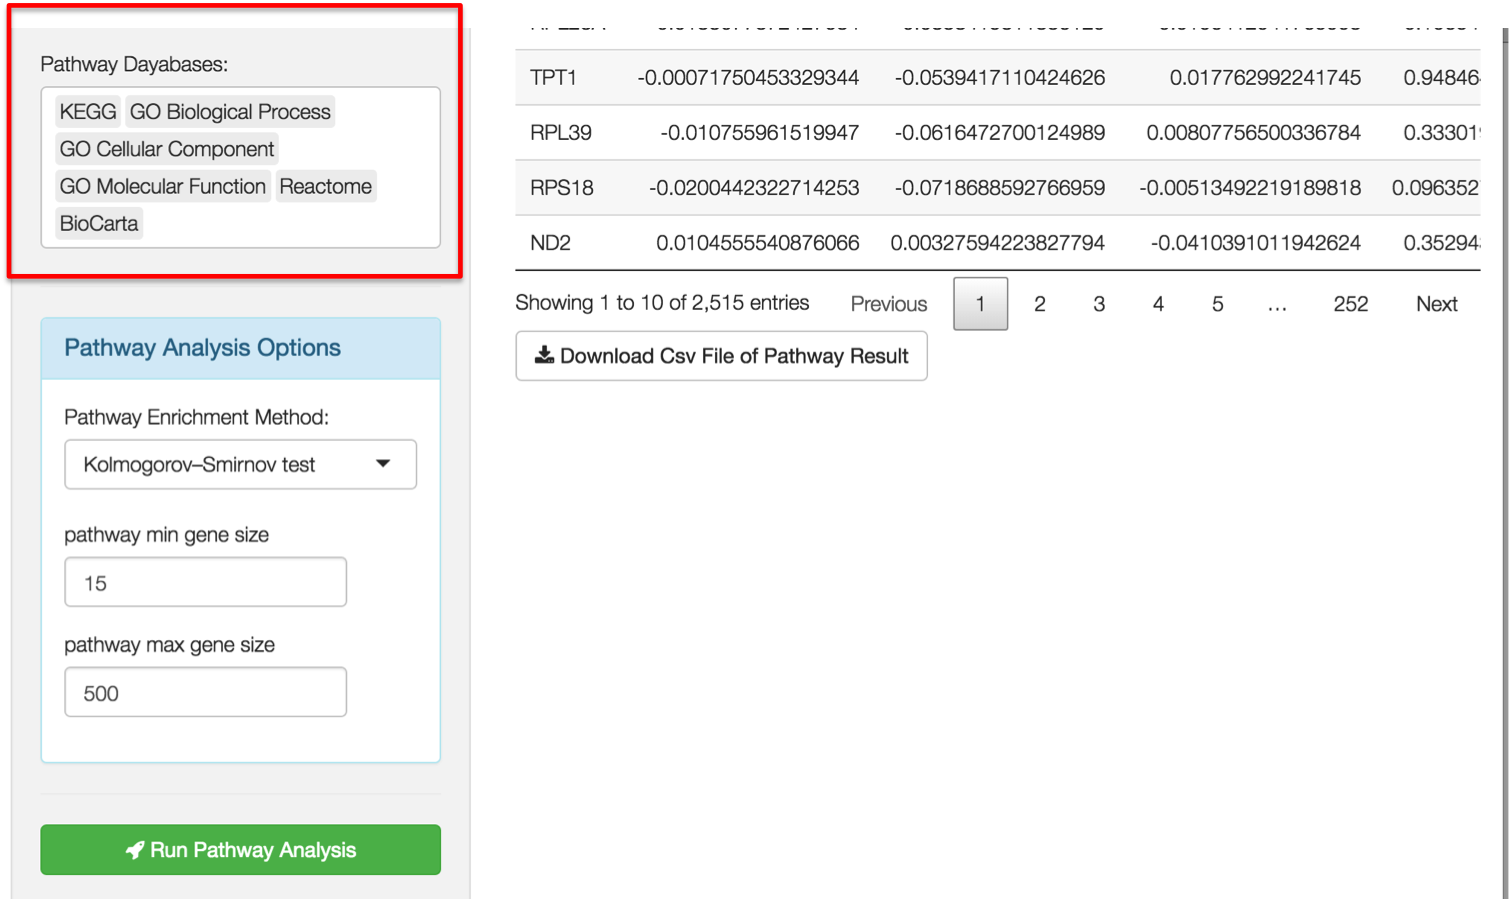
\includegraphics[scale=0.45]{./figure/metaDE/PathwayDB}
\caption{Selection of pathway database}
\label{fig:PathwayDB}
\end{center}
\end{figure}

\begin{figure}[H]
\begin{center}
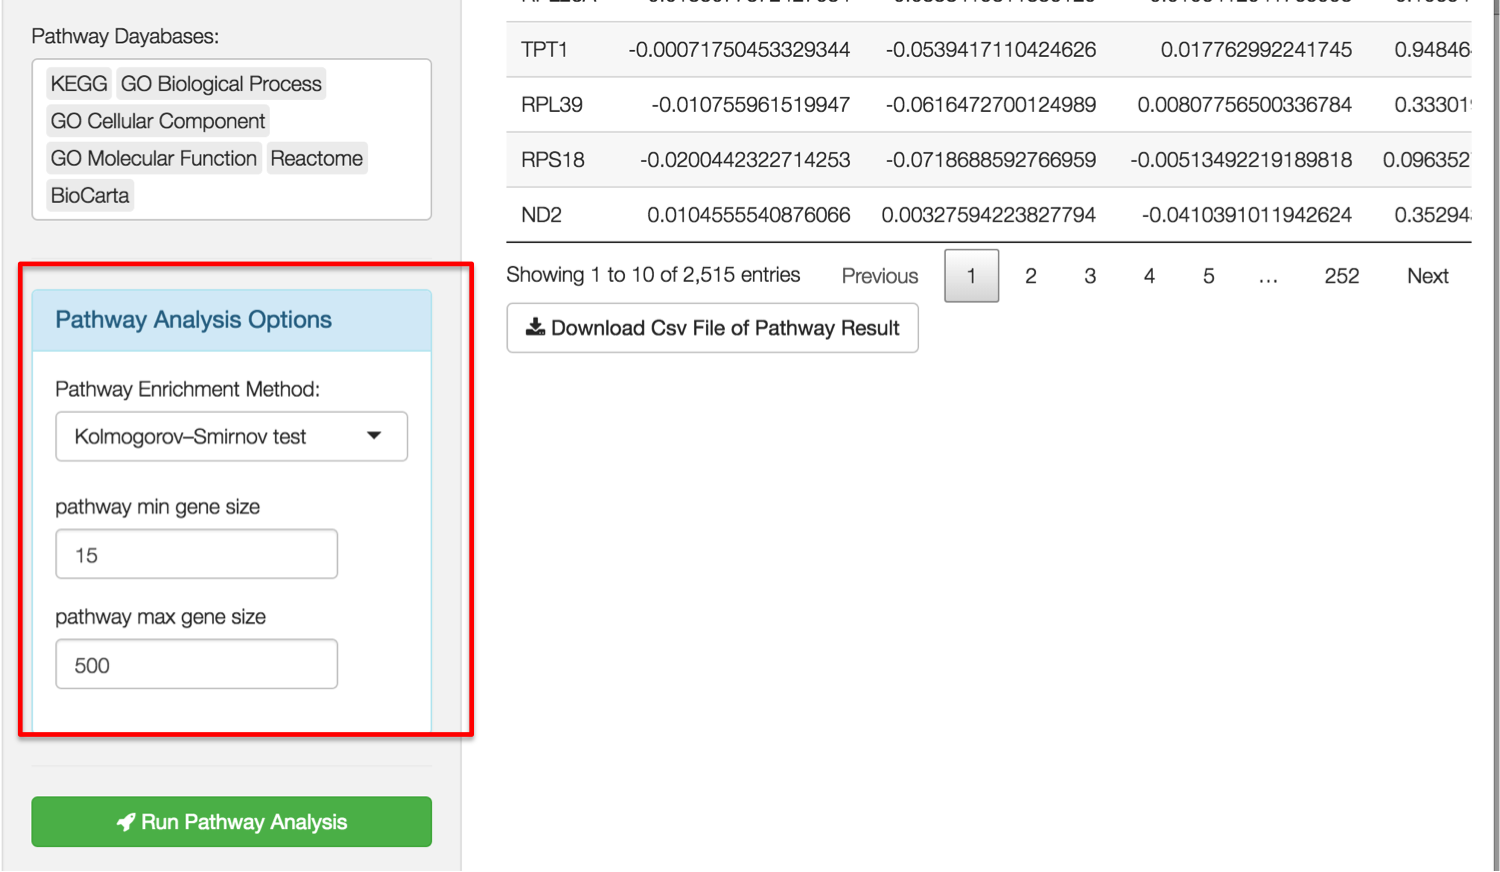
\includegraphics[scale=0.45]{./figure/metaDE/KStest}
\caption{KS test setting}
\label{fig:KStest}
\end{center}
\end{figure}

\begin{figure}[H]
\begin{center}
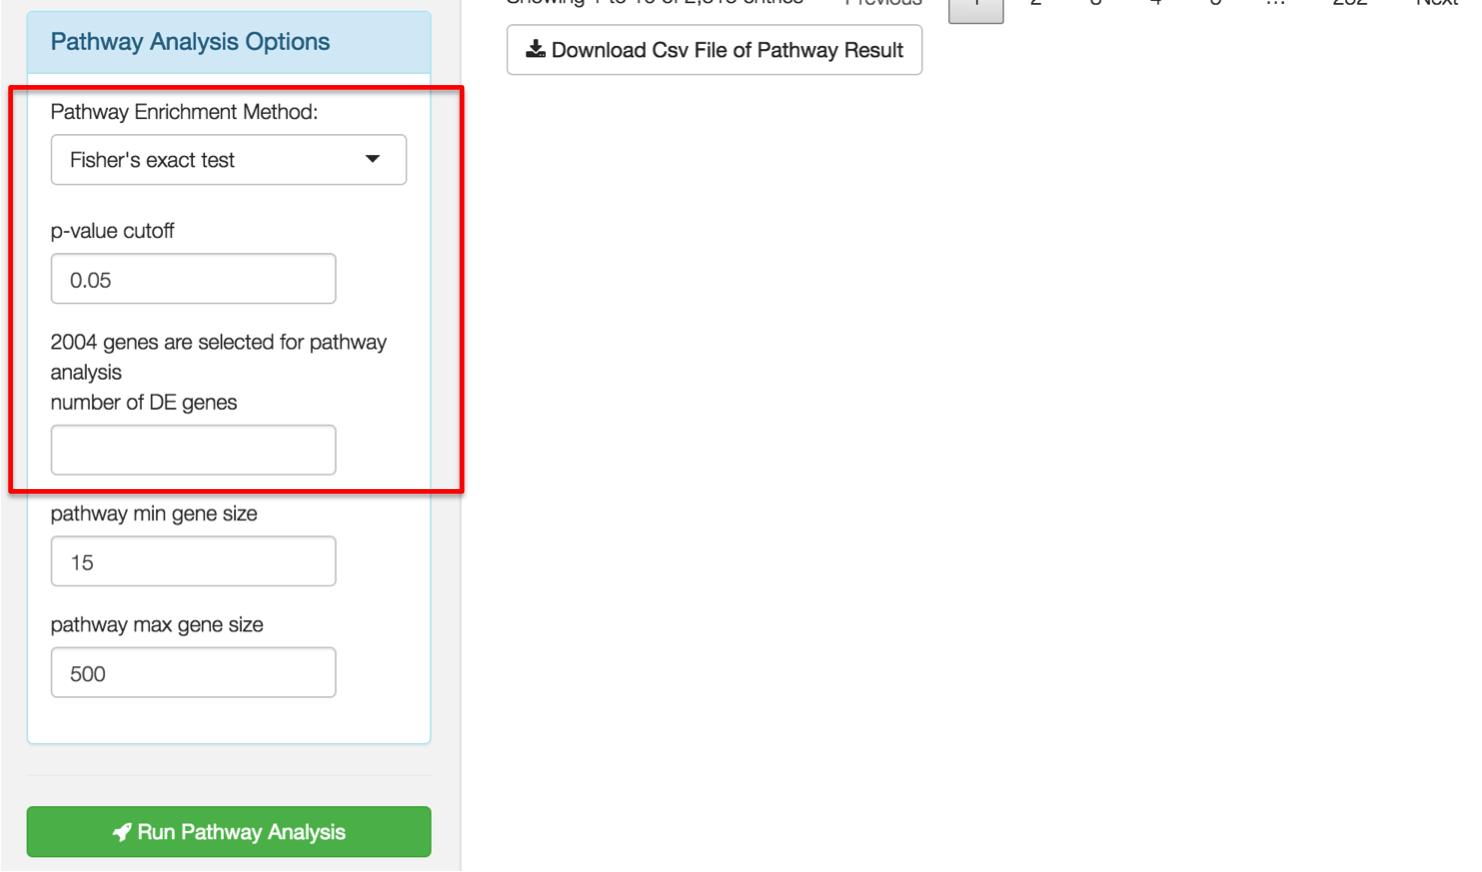
\includegraphics[scale=0.45]{./figure/metaDE/FisherExact}
\caption{Fisher's exact test setting}
\label{fig:FisherExact}
\end{center}
\end{figure}

We will then see a summary table of pathway analysis results generated on the right of the page as shown in Figure \ref{fig:PathResult}. Users can search the pathway name in the ``Search" bar, and download the full table as a csv file by clicking on ``Download Csv File of Pathway Result" as highlighted. 

\begin{figure}[H]
\begin{center}
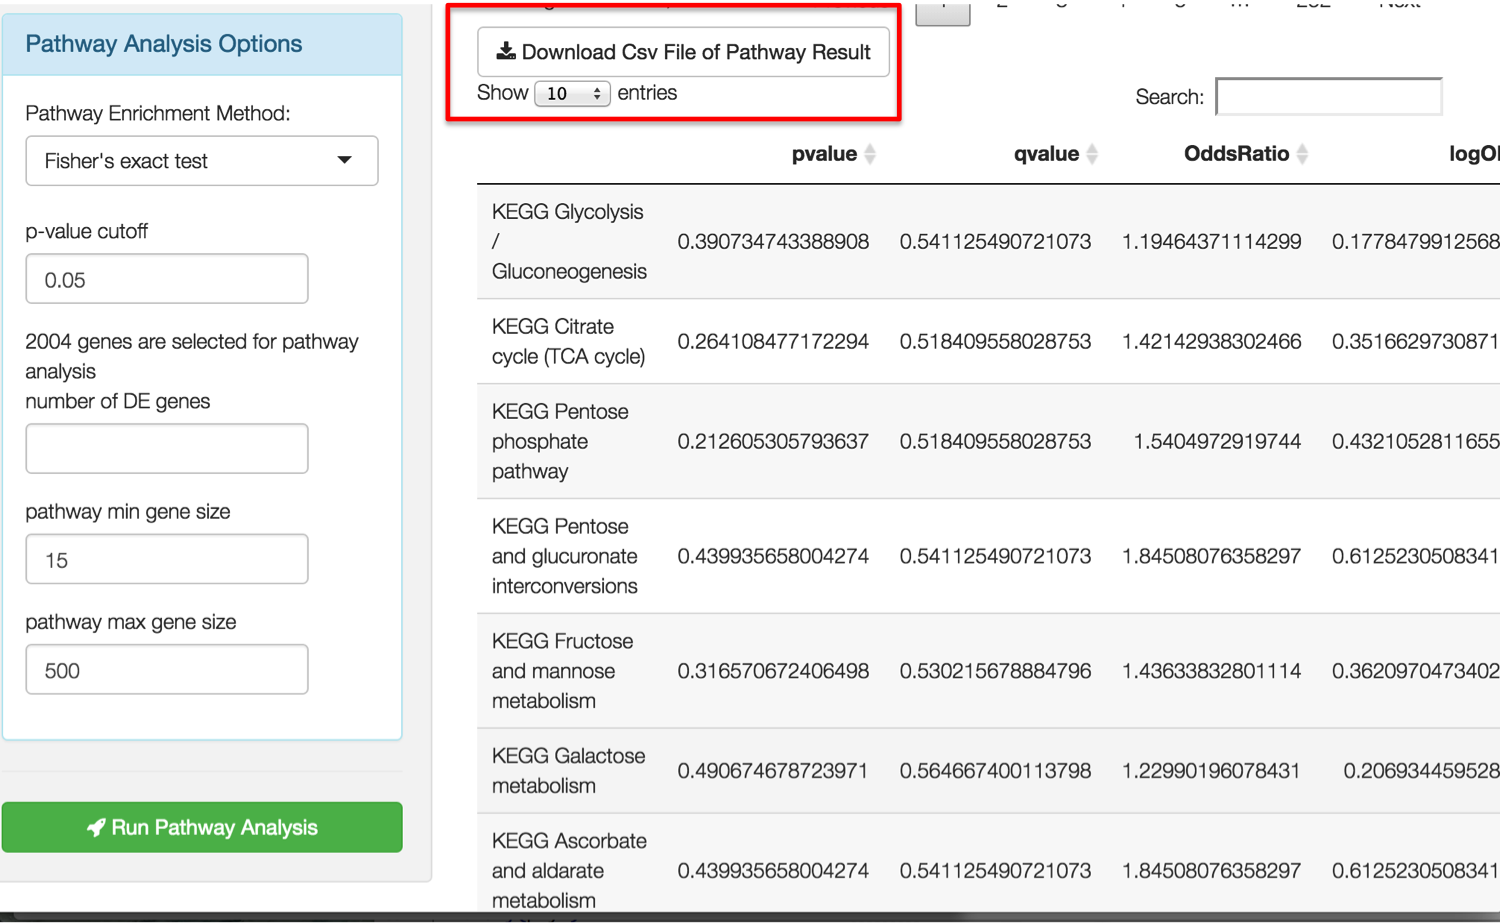
\includegraphics[scale=0.45]{./figure/metaDE/PathResult}
\caption{Summary of pathway analysis result}
\label{fig:PathResult}
\end{center}
\end{figure}
